\documentclass[12pt,letterpaper]{article}
\usepackage[latin1]{inputenc}
\usepackage{amsmath}
\usepackage{amsfonts}
\usepackage{amssymb}
\usepackage{multicol}
\usepackage{graphicx}
\usepackage{wrapfig}
\usepackage{amsmath}
\begin{document}
\title{Ionospheres Assignment 1}
\author{Jonathan Nickerson}
\date{January 17, 2012}
\maketitle
\begin{abstract}
The purpose of this assignment is to build a simple model of the neutral thermosphere in hydrostatic equilibrium. The model I used and the results of that model are discussed\footnote{This project was a first for me in two ways: 1) It is the first program/model I have ever written and 2) This is the first document I have ever typed using LaTeX. While the program ended up being a HUGE success, I feel this document is lacking a bit in sophistication and detail. Thus I ask that you be forgiving this week in recognition that my writeups should improve with time.}.
\end{abstract}
%\begin{multicols}{2}
%\end{multicols}
\section{The Model}
The neutral atmosphere above \raise.17ex\hbox{$\scriptstyle\sim$}100km can be modeled to a good approximation under hydrostatic equilibrium as:

\begin{equation}
	n_{s}(z)=n_{s}(z_{0})\frac{T(z_{0})}{T(z)}\exp \bigg(-\frac{\Delta z}{H}\bigg) 
\end{equation}

\noindent where 

\begin{equation}
	H=\frac{k_{B}\Delta T}{m_{s}\Delta g}
\end{equation}

\noindent and the change in gravity with altitude is calculated by

\begin{equation}
	\Delta g=g_{0}\bigg(\frac{R_{E}}{R_{E}+z}\bigg)^2
\end{equation}

The temperature varies from 200K to 1000K reaching its peak around 350km and is given as:

\begin{equation} \label{eq:T1}
	T = 800.0*\tanh(\theta*3.0)+200.0
\end{equation}

\noindent In this way we can numerically calculate the number density of each species at every step in altitude. 

The neutral atmosphere is dominated by eddy diffusion (well mixed) to an altitude of \raise.17ex\hbox{$\scriptstyle\sim$}120km. To simulate this I used a mass density weighted scale height for all species from 100km - 120km. Above 120km molecular diffusion begins to dominate so each species assumes it's own scale height.

\section{The Results}

The above described model calculates 1000 steps over an altitude range from 100km to 800km. It can be seen in Figure~\ref{fig:Density vs Altitude 1} that the model behaves as expected in that at low altitudes the atmosphere is dominated by N2 and then rapidly submits to molecular oxygen as the dominant species around 300km. Tamas Gombosi's book "Physics of the Space Environment" implies that atomic oxygen becomes the major constituent at closer to \raise.17ex\hbox{$\scriptstyle\sim$}200km altitude. So this model may require some improvement. None the less I feel this is a reasonably happy first approximation and overall the model does yeild the expected slopes for each species.

To demonstrate that the slopes of each species in Figure~\ref{fig:Density vs Altitude 1} are in fact identical to each other over the altitude range from 100km to 120km I asked the model to plot Figure~\ref{fig:Density vs Altitude 2} which shows the altitude range from 100km to 140km in closer detail. Plotting all of the scale heights together in Figure~\ref{fig:Scale Height vs Altitude 1} also reinforces this point. As expected the scale heights of each species appear in order by mass. This also indicates that if I had plotted this model to altitudes greater than 800km eventually atomic nitrogen would overtake atmic oxygen as the major constituent. In reality I do not believe atomic nitrogen is a major constituent at any altitude in the thermosphere.

The model also plots the mass density as it varies with altitude. What I found was that the slopes are very similar but not identical (Figure~\ref{fig:Mass Density vs Altitude 1}).  

As previously mentioned Equation \eqref{eq:T1} allows the temperature to vary from 200K to 1000K reaching its peak near 350km (Figure~\ref{fig:Temperature vs Altitude 1}). Naturally, the next thing to do with this model was to change the parameters of Equation \eqref{eq:T1} and see how this changed the behavior of the thermosphere. Allowing the temperature to increas more rapidly:

\begin{equation} \label{eq:T2}
	T = 800.0*\tanh(\theta*9.0)+200.0
\end{equation}

\noindent causes a rather dramatic change in the scale heights. The consequences can be seen in Figure~\ref{fig:Temperature vs Altitude 2}, Figure~\ref{fig:Scale Height vs Altitude 2}, and Figure~\ref{fig:Density vs Altitude 3}.

Tweaking the gravitational parameter within the scale height will cause a change in the structure of the thermosphere. For example if we were to hold standard gravity constant and double the radius of the Earth, the gravitational parameter would go as:

\begin{equation}
	\Delta g=g_{0}\bigg(\frac{2R_{E}}{2R_{E}+z}\bigg)^2
\end{equation}

\noindent this would steepen the slope of the scale heights. A more exagerated example of this is shown in Figure~\ref{fig:Scale Height vs Altitude 3} in which the radius is 20x that of the Earth.

Lastly, another very interesting plot to look at is the total weighted molecular mass vs altitude (Figure~\ref{fig:Total Weighted Molecular Mass vs Altitude 1}). This demonstrates that the weighted molecular mass of the thermosphere at lower altitudes is closer to that of N2 and slowly decreases with height. As the heavier constituents fall off with altitude the weighted molecular mass approaches that of molecular oxygen (Note the purely vertical slope from 100km - 120km).

\section{Conclusion}

This was a rich, enjoyable learning experience. I look forward to continuing to improve upon this model through out the rest of the semester as I continue to sharpen my programing and typesetting skills.

\begin{figure*}[htb]
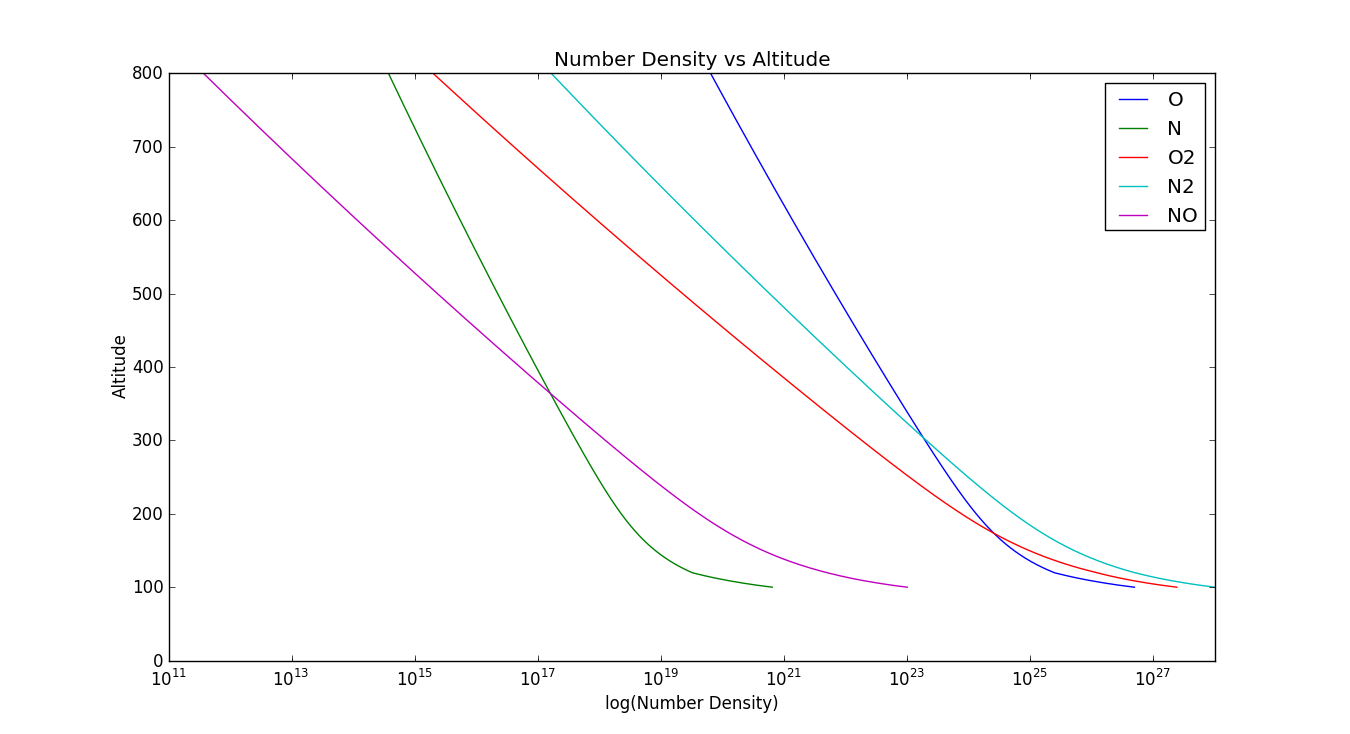
\includegraphics[scale = .40, keepaspectratio]{Figures/Density_vs_Altitude_100_800.png}
\caption{The slopes of the number densities give the expected behavior with altitude.}
\label{fig:Density vs Altitude 1}
\end{figure*}

\begin{figure*}[htb]
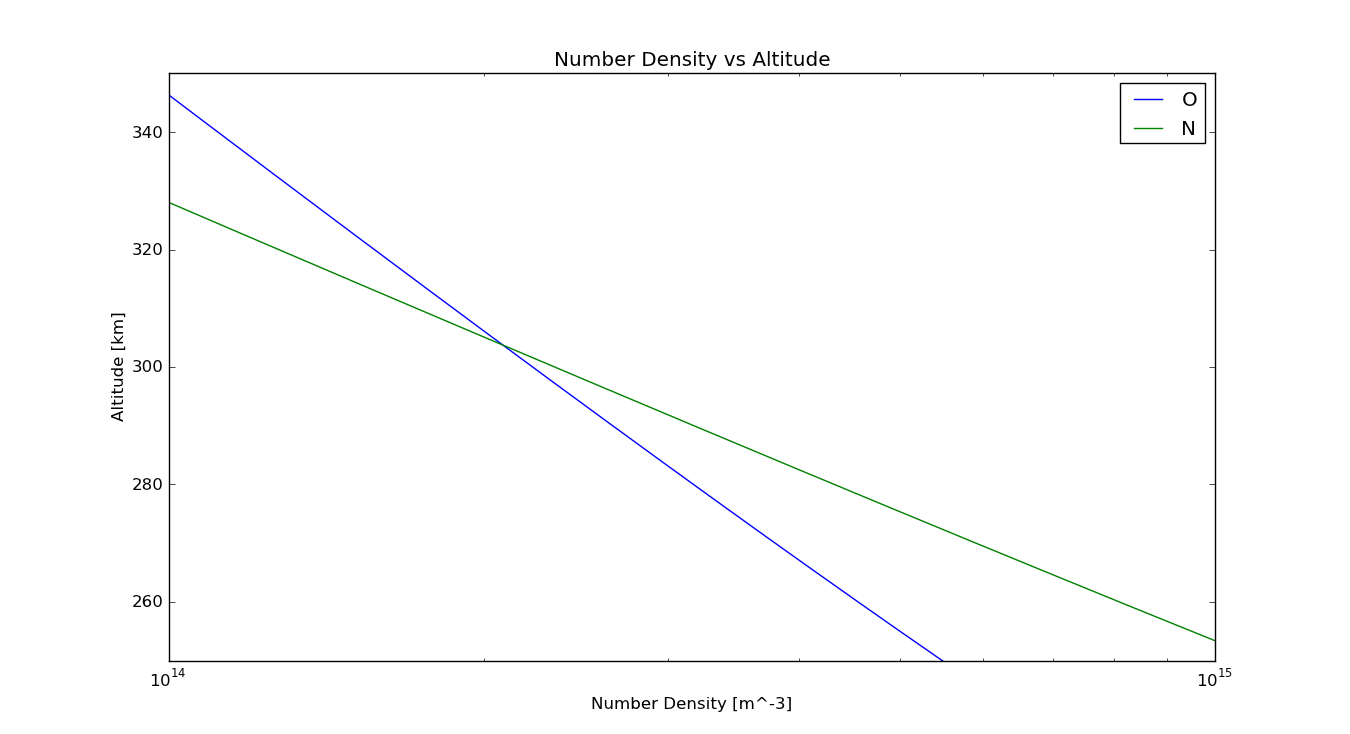
\includegraphics[scale = .40, keepaspectratio]{Figures/Density_vs_Altitude_100_200.png}
\caption{The slopes of the number densities are in fact the same up to 120km.}
\label{fig:Density vs Altitude 2}
\end{figure*}

\begin{figure*}[htb]
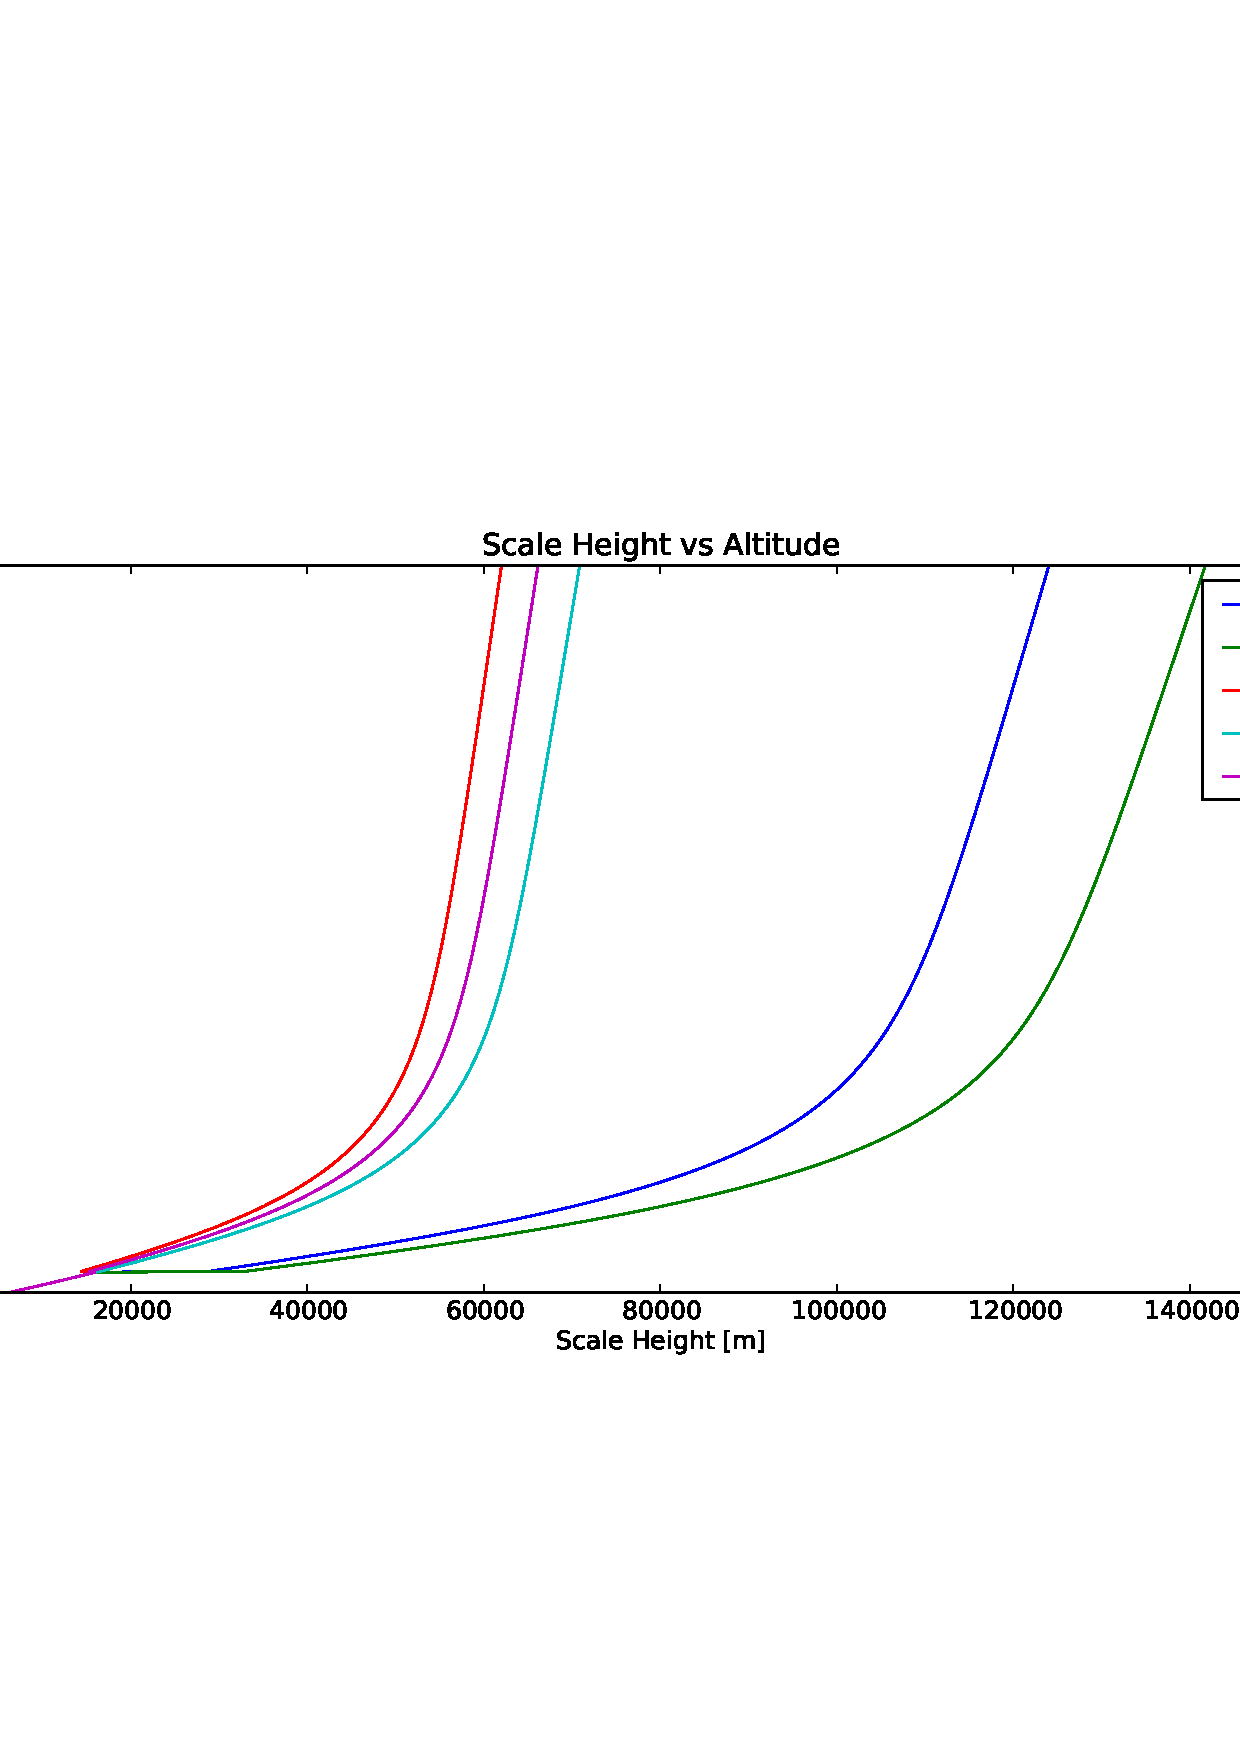
\includegraphics[scale = .40, keepaspectratio]{Figures/Scale_Height_vs_Altitude.png}
\caption{The scale heights of each species show good mass dependence.}
\label{fig:Scale Height vs Altitude 1}
\end{figure*}

\begin{figure*}[htb]
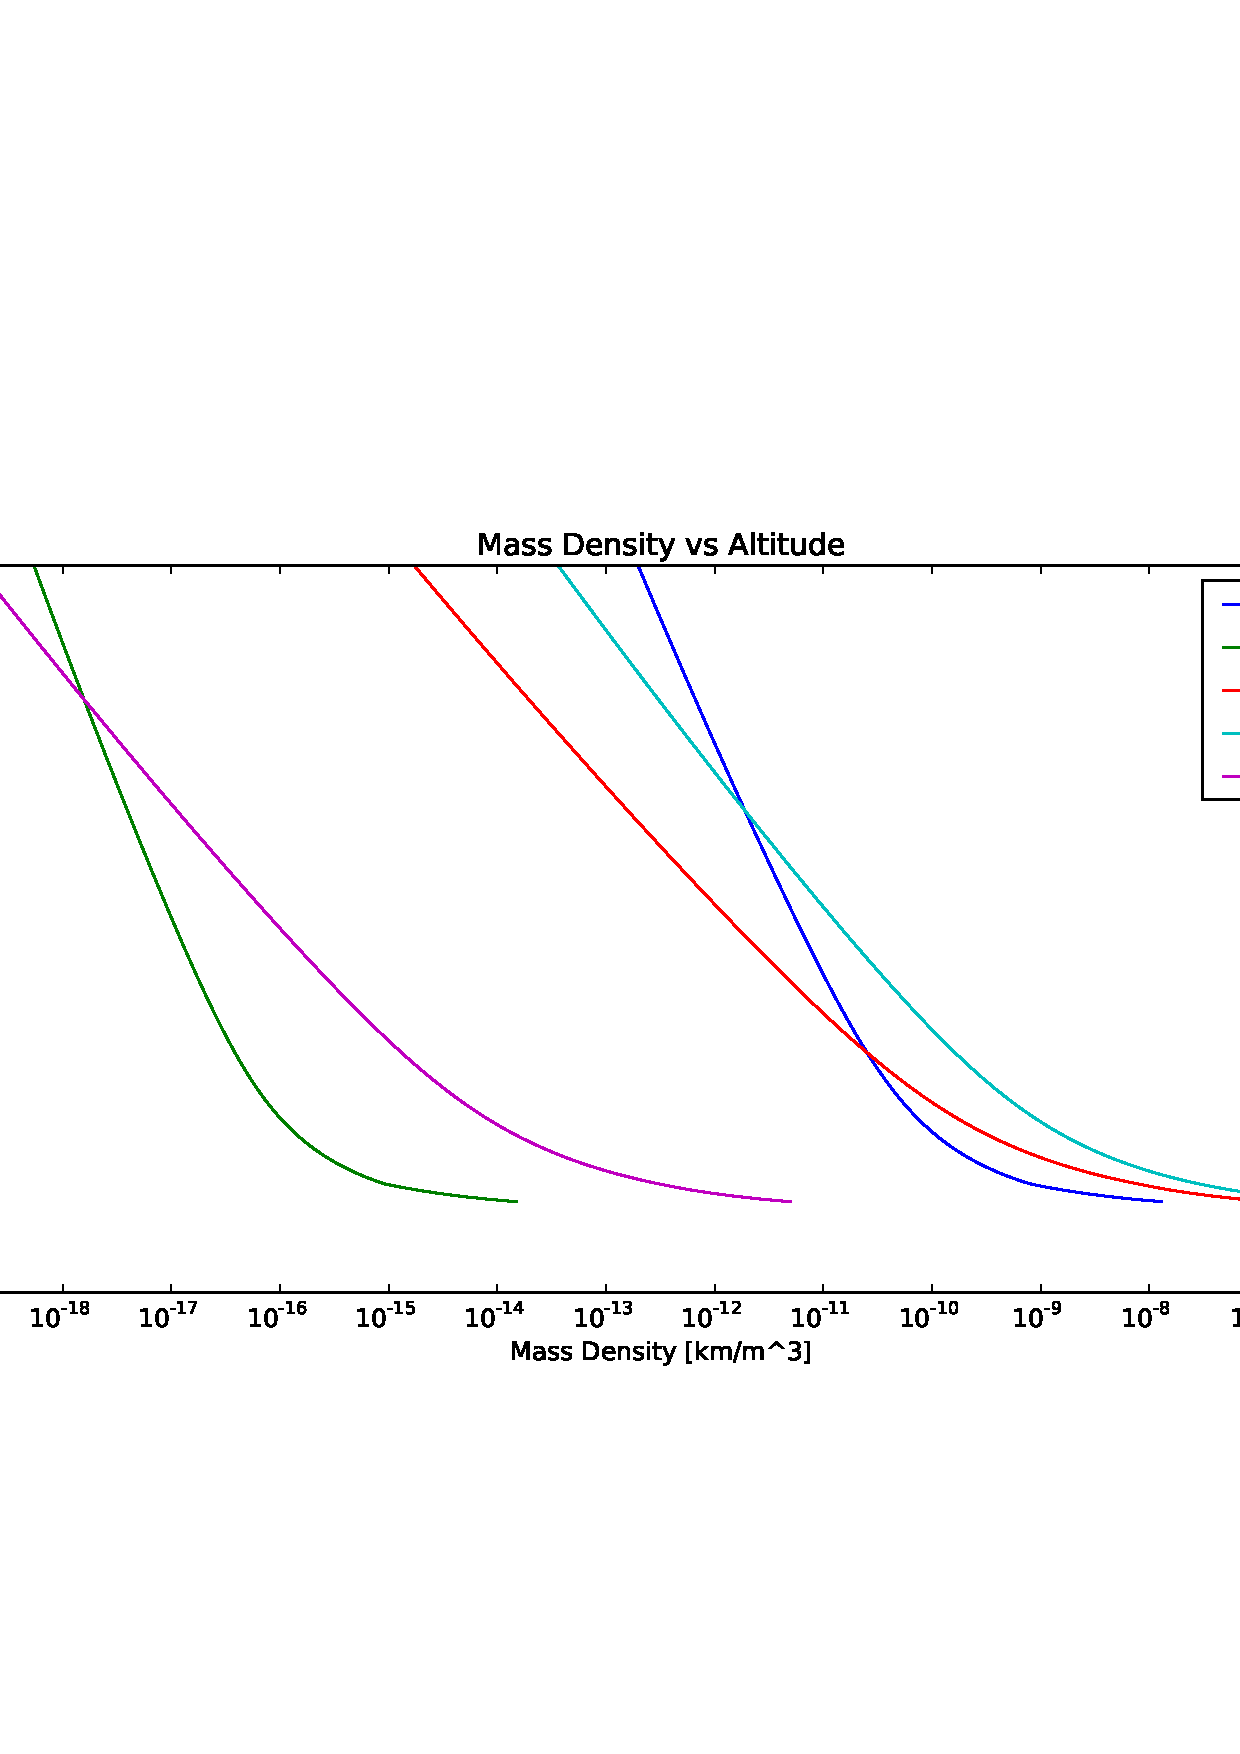
\includegraphics[scale = .40, keepaspectratio]{Figures/Mass_Density_vs_Altitude.png}
\caption{Mass density shows similar, but not identical, behavior to number density.}
\label{fig:Mass Density vs Altitude 1}
\end{figure*}

\begin{figure*}[htb]
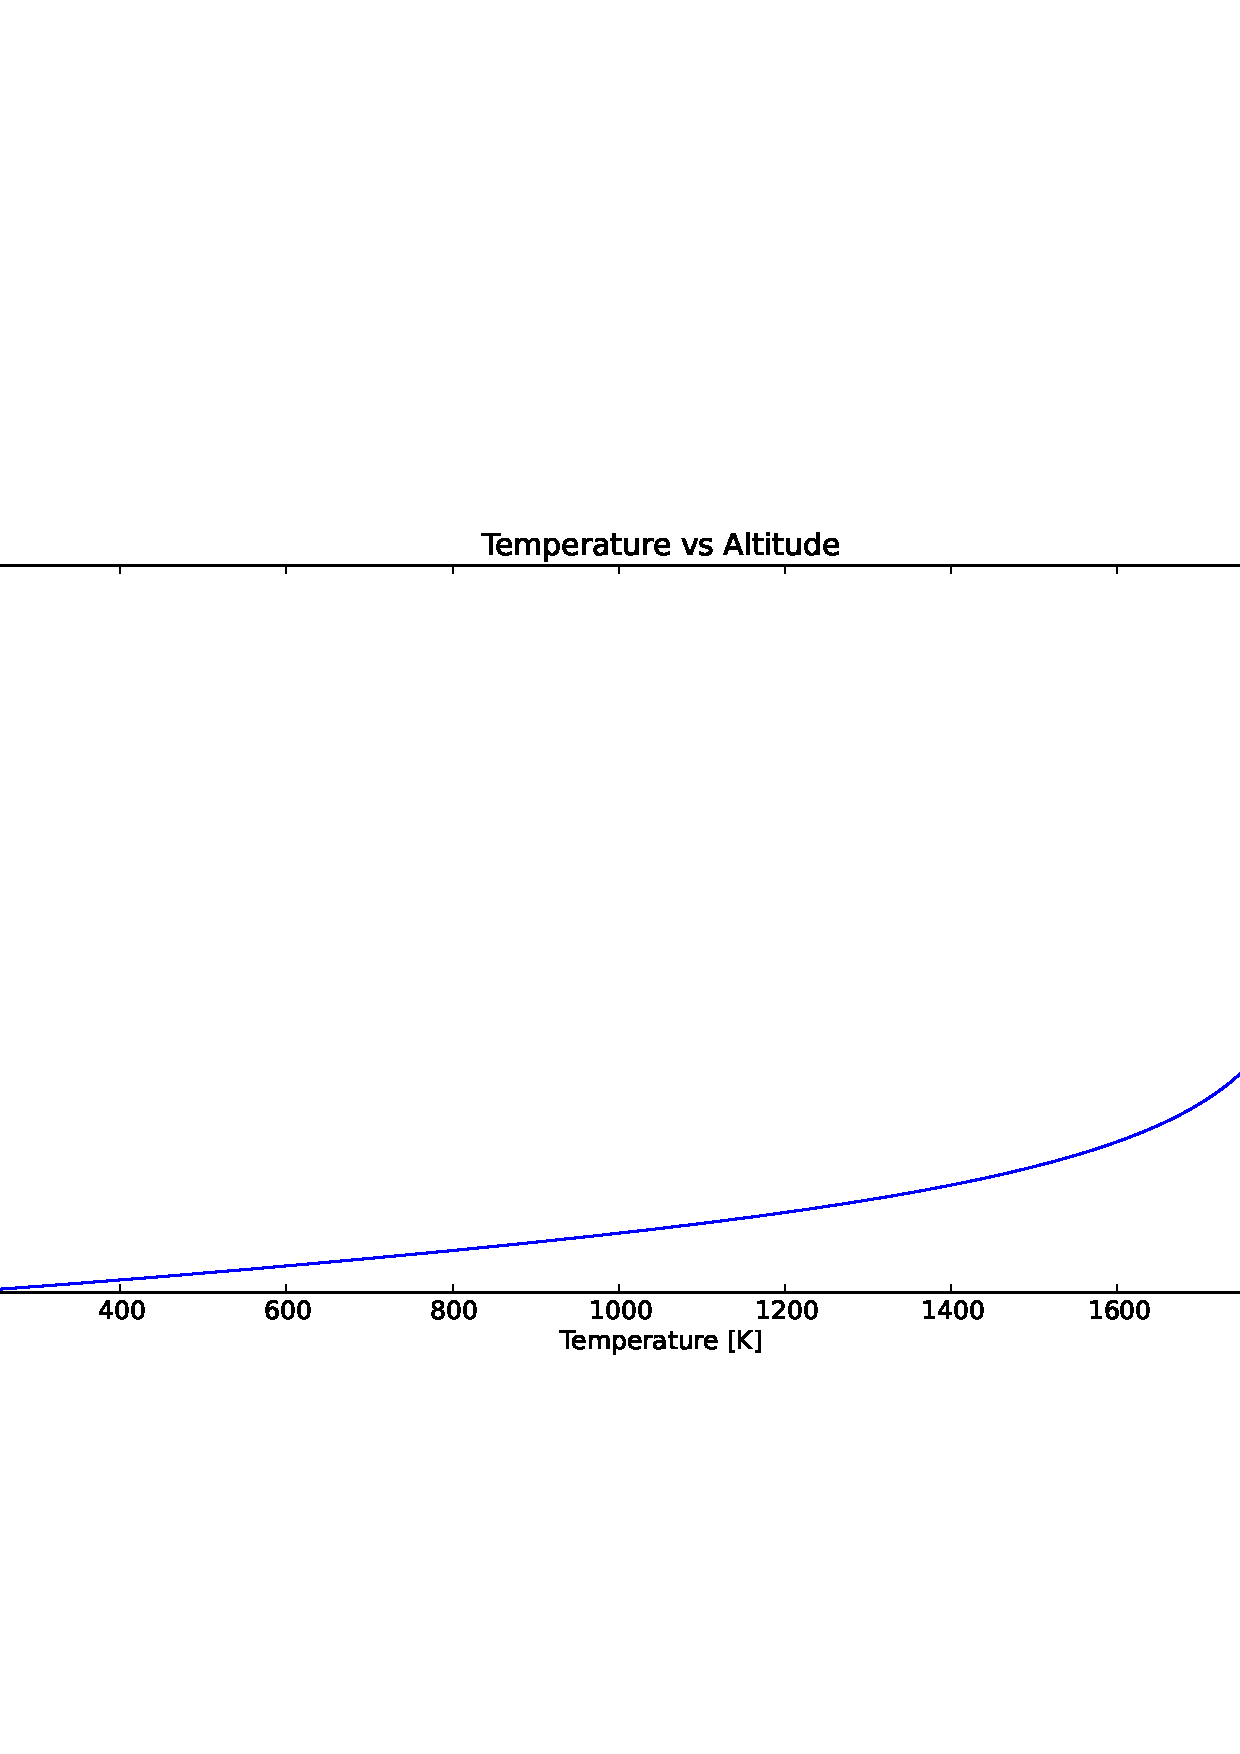
\includegraphics[scale = .40, keepaspectratio]{Figures/Temperature_vs_Altitude.png}
\caption{The temperature reaches a maximum value near 350km.}
\label{fig:Temperature vs Altitude 1}
\end{figure*}

\begin{figure*}[htb]
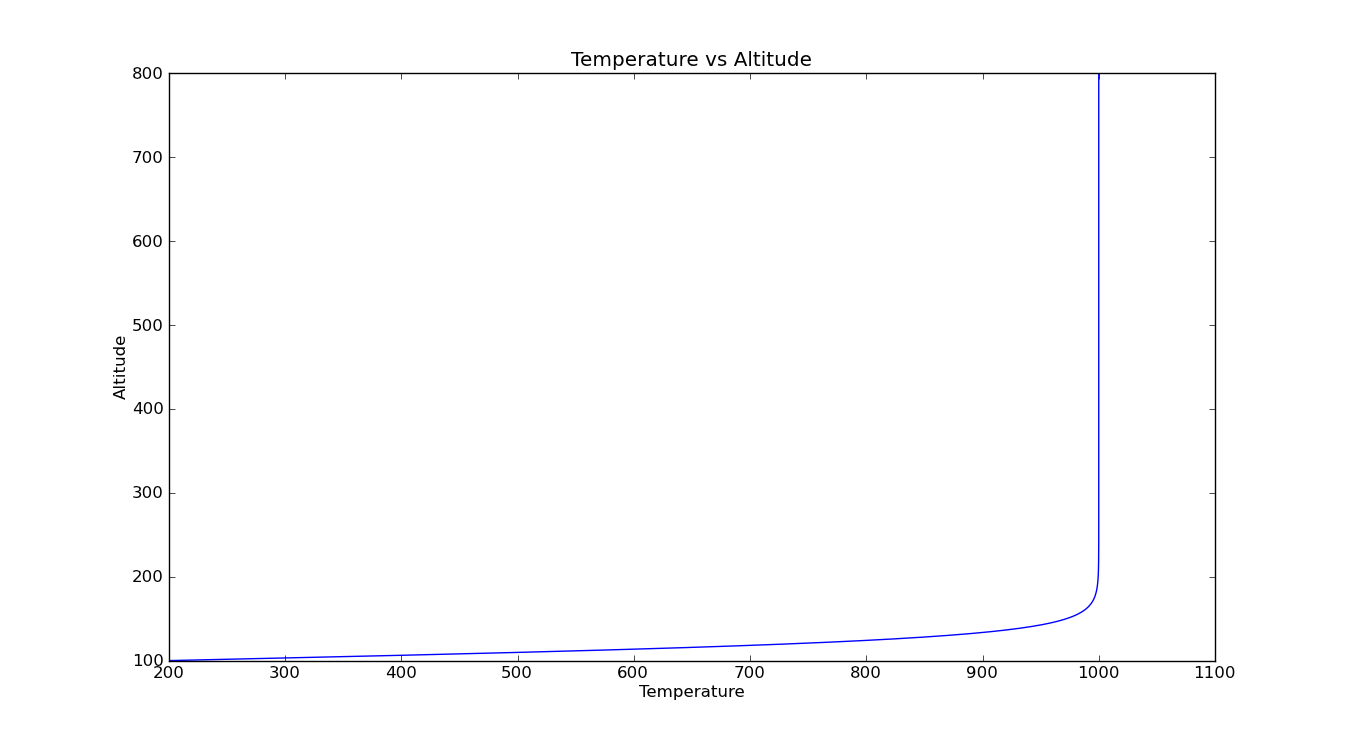
\includegraphics[scale = .40, keepaspectratio]{Figures/Temperature_vs_Altitude_New_Temp.png}
\caption{The new temperature profile reaches a maximum value much sooner.}
\label{fig:Temperature vs Altitude 2}
\end{figure*}

\begin{figure*}[htb]
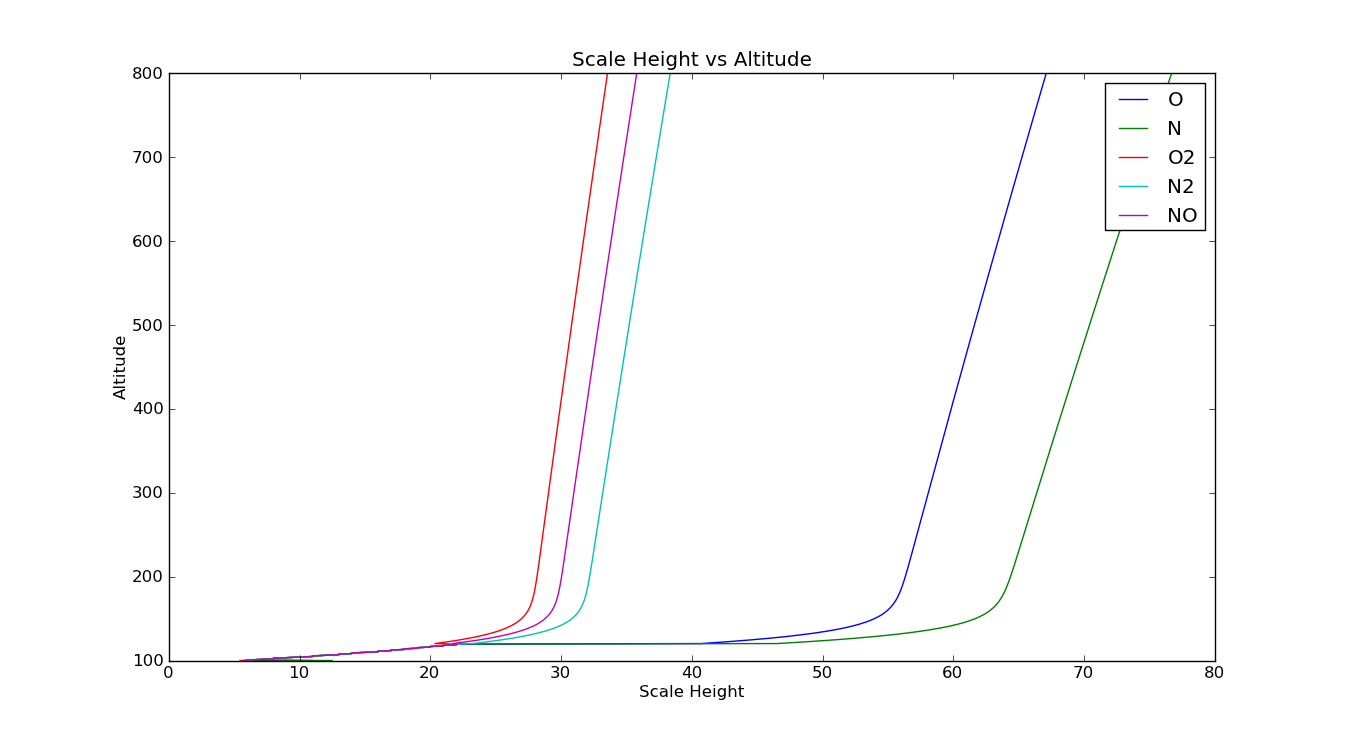
\includegraphics[scale = .40, keepaspectratio]{Figures/Scale_Height_vs_Altitude_New_Temp.png}
\caption{The scale heights increase faster at lower altitude with the new temperature profile.}
\label{fig:Scale Height vs Altitude 2}
\end{figure*}

\begin{figure*}[htb]
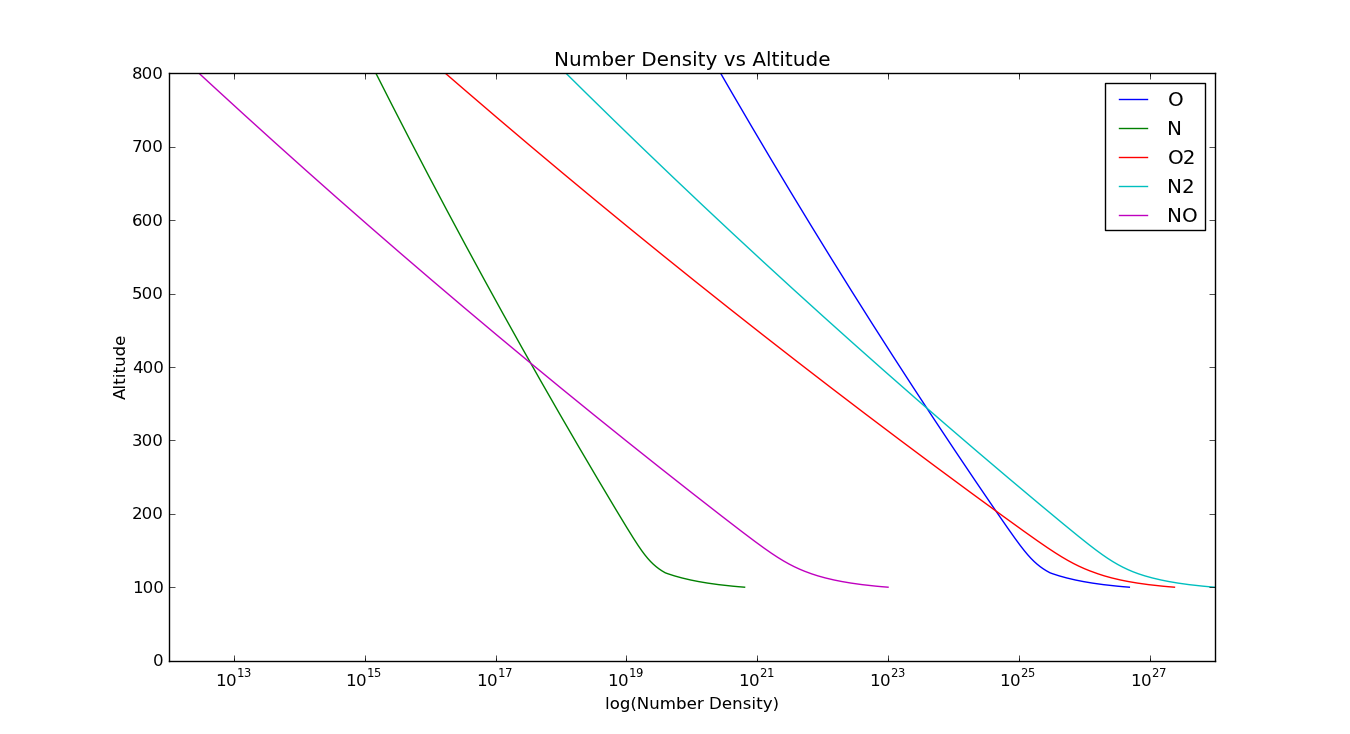
\includegraphics[scale = .40, keepaspectratio]{Figures/Density_vs_Altitude_New_Temp.png}
\caption{New scale heights change the slopes of the number densities.}
\label{fig:Density vs Altitude 3}
\end{figure*}

\begin{figure*}[htb]
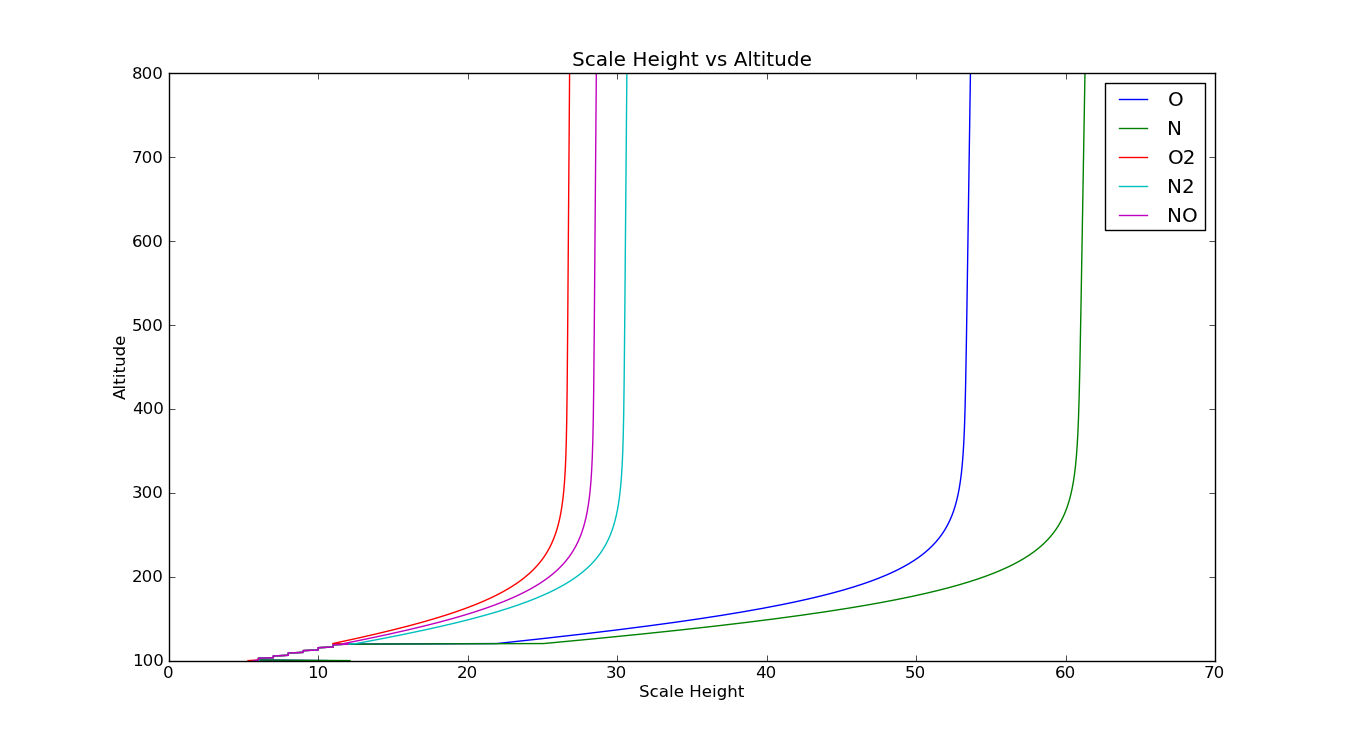
\includegraphics[scale = .40, keepaspectratio]{Figures/Scale_Height_vs_Altitude_Grav.png}
\caption{With increase in planetary radius the slope of the scale heights steepen.}
\label{fig:Scale Height vs Altitude 3}
\end{figure*}

\begin{figure*}[htb]
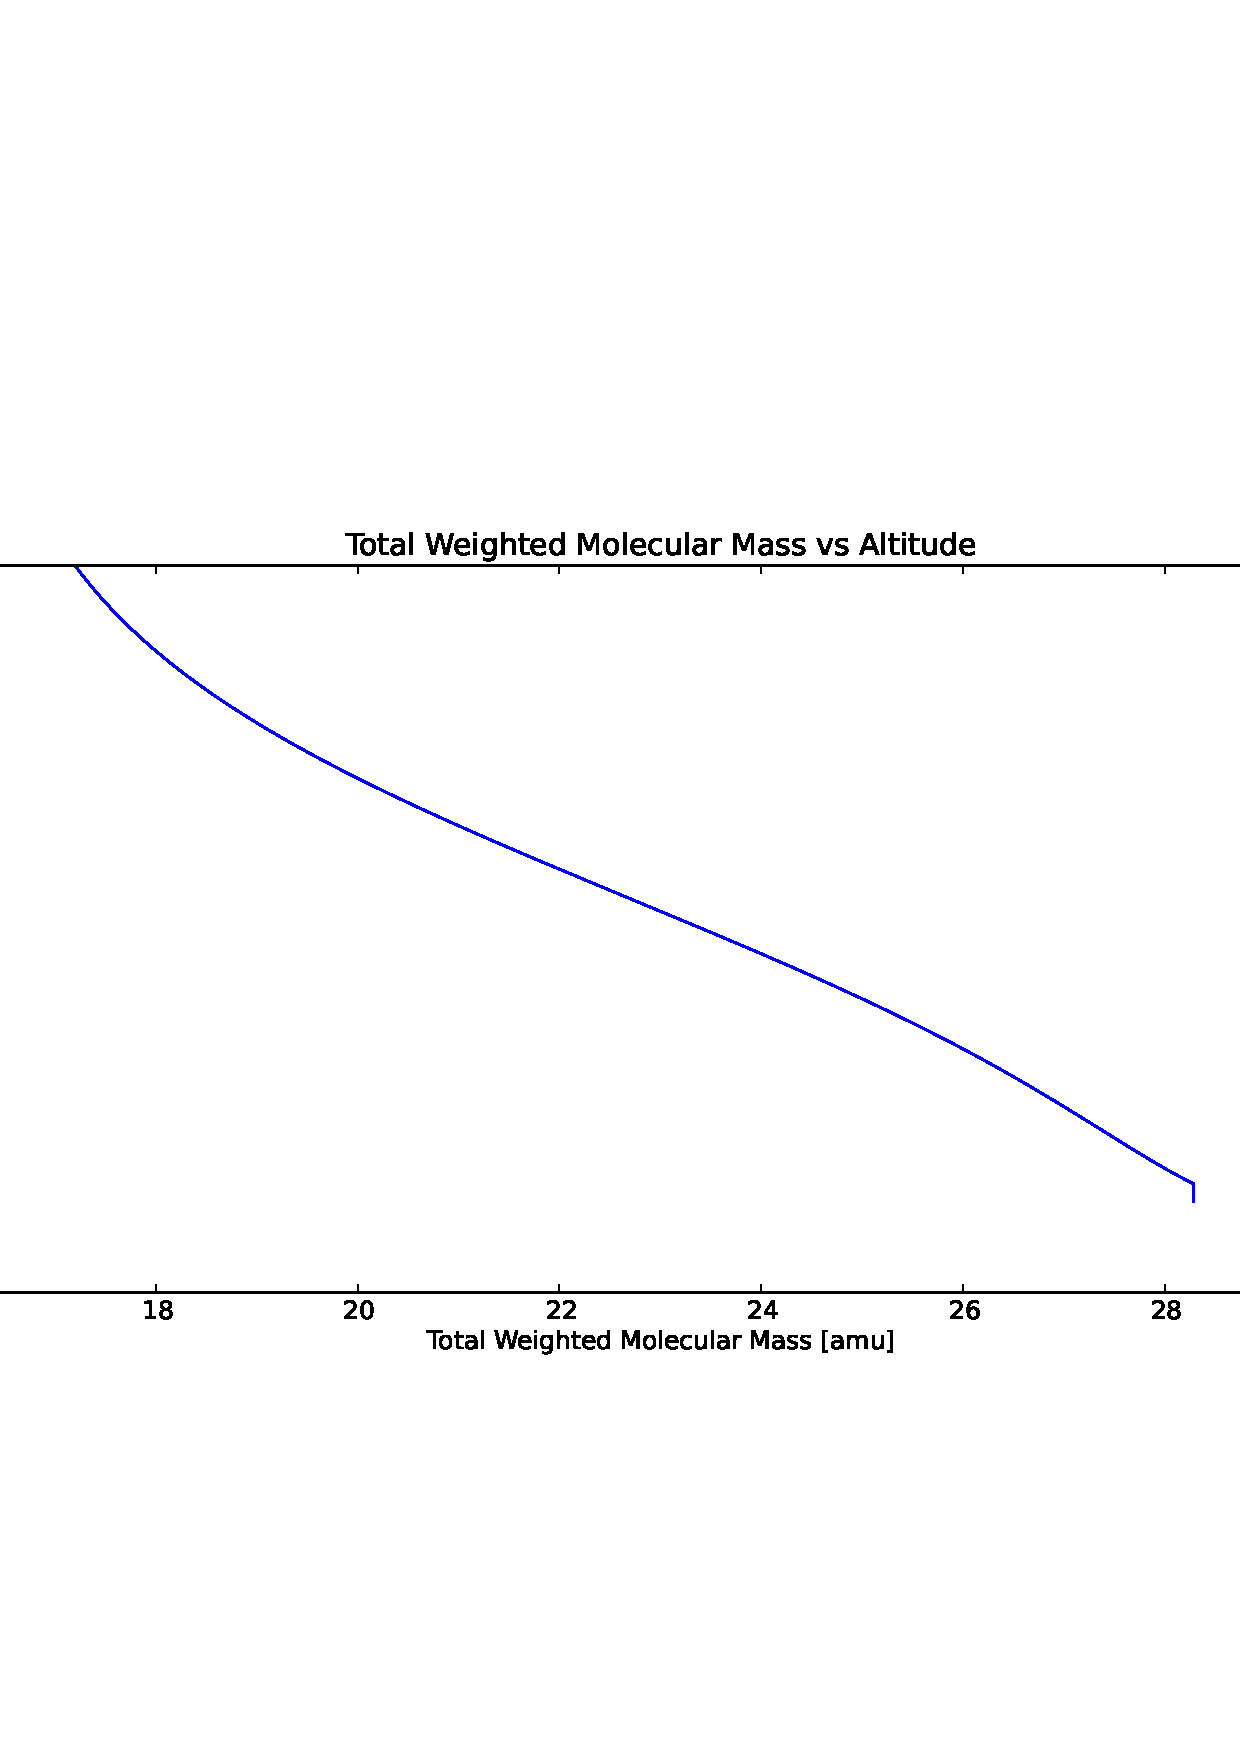
\includegraphics[scale = .40, keepaspectratio]{Figures/Total_Weighted_Molecular_Mass_vs_Altitude.png}
\caption{The weighted molecular mass composition is near that of N2 in the lower altitudes and decreases with altitude approaching a mass close to that of molecular oxygen at higher altitudes.}
\label{fig:Total Weighted Molecular Mass vs Altitude 1}
\end{figure*}





\end{document}